%!TEX root = project.tex

\chapter*{About this project}
\paragraph{Abstract}

This project was contracted to us through Enterprise Ireland from a company called RoamPA founded by Una McNeill. RoamPA contacted us to build two modules for a J2EE (Java Enterprise Edition) web application. RoamPA was building a web application aimed at business users and contracted two modules to be developed for them externally. One of the modules consisted of converting an already existing legacy reports module so it would work in a Tomcat environment. This module would allow administrator users to create reports using a streamlined query builder. This system was primarily aimed at administrator users from the human resources department. The other module 
was a reviews system. The reviews system allows users to generate reviews about existing businesses,faculties, points of interest etc. The reviews system would also let users create,update,view,like and dislike reviews, similar to Trip Advisor. Both of these modules had to be created from scratch and had to integrate into RoamPA's existing server environment. This integration restrains the technologies used and furthermore required the modules to be integrable with their RDMBS (Relational Database Management System). The project involved research, learning many frameworks and understanding the architectural patterns involved with developing a J2EE application.

\paragraph{Authors}

The authors of this project are Andrew Sweeney and John Frizzell. We are both graduates of the BSc in Computing in Software Development which was the preceding course to the current honors degree. We both have a great interest in programming and technology. We are constantly seeking ways to improve our knowledge and skills.


\chapter{Introduction}

RoamPA Ltd is a start-up company founded by Una McNeill. They are developing a web application which is used to streamline the process of moving employees globally for work and business purposes. They wish to provide a much improved employee experience, significant cost savings to clients and greater return on investments with assignments and business travel.

We had previously worked with Una McNeill through another Enterprise Ireland contract. The previous contract involved creating a reports module and involved four students altogether. Our last project was our first real collaborative experience where we programmed together whilst incrementally updating the project. This project was delivered successfully to RoamPA and served to build a relationship which acquired us a further contract. 

Creating the previous report module was our first real experience with developing in web and server languages such as PHP and JavaScript. The reports module is now a legacy module because the environment for the web application had now shifted from a PHP MVC web application (Model View Controller) environment to now a J2EE web application environment. This shift in environments meant having to redo the reports module as the server language used was now Java and not PHP. Recreating the reports module was one of the two modules we had to produce.

The main module we had to create was a reviews module. This again was restrained by the current environment and involved a lot of researching and agile iterative development. The reviews module consisted of a map element and being able to add reviews to filtered establishments that populated the map. This system would be used to view and create reviews. Based off a reviews popularity or recommendation an employee could judge whether or not to give their business to the reviewed establishment.

\newpage

\chapter{Context}

\section{Why we chose this project}

Throughout our college course we have developed in many different languages. Java, C\#, C and Python to name a few. We have not had the chance to really to dig deeply into web development. Web languages like PHP and JavaScript were not part of our syllabus. Our sister course "Computing in Digital Media" does some of the design elements of web development but not much of the back-end stuff that we've both liked. Throughout our course we had a few semesters that had Database modules involving MYSQL. We heard the current project involved full blown MVC, Servlets, ORM and JSP pages. We also learned that the main language required for the project was Java which is one of the core languages for our college course. This project gave us a whole new area to experiment with and learn. The project would give us the opportunity to develop for a J2EE environment. Due to the challenge and interest we accepted the contract for nthis project.

\section{Challenges we had to face}    

Straight from the beginning, the challenge was to understand all of the frameworks and how all of the different parts of the environment work together. This meant completely understanding concepts like ORM and how they are applied through the framework Hibernate. Other concepts included learning how MVC is applied through SpringMVC with routes etc. There was a lot to research and a lot of frameworks to read up on. There was also numerous dependencies to figure out. The amount of research, tutorials and understanding to be put into the project was also a big challenge as well as the actual development of the project itself. 


\section{Objectives}

\begin{itemize}
\item{Follow the specifications provided to make integration easier}
\item{Research the frameworks and environment}
\item{Create a reports module}
\item{Create a reviews module}
\end{itemize}

\section{Specifications}

We were creating two modules for RoamPA. Both modules had to be integrated onto RoamPA's existing Application server. The Frameworks required of us were to use Hibernate ORM and SpringMVC. The existing database RoamPA uses is MySQL. All of the code handed over to RoamPA must be integrable on their server.

The first module involved creating a reviews system. The reviews system should allow the customer to look up an area using a search box and using filters then find locations for buildings like hospitals,restaurants and numerous other points of interest. The customer could then click on the Point of Interest (POI) and create a review for a business. They can also rate a current review that exists on there and like or dislike it.

The second module \newline

\textbf{JOHNS BIT ABOUT REPORT GENERATOR}


\chapter{Methodology}
We used a form of the Agile development methodology on this project, with iterative prototyping, team VOIP calls, and weekly meetings with our project supervisor/manager as well as frequent meetings and communication with the clients. We used git as our version control system with our repositories being hosted on GitHub.

\section{Orientation Sprints}
(Sprint: \emph{A time period (typically 1–4 weeks) in which development occurs on a set of backlog items that the team has committed to—commonly referred to as a time-box or iteration}) 
Our Development of the main Orientation module essentially breaks down into 6 sprints:

\subsection{Sprint  1: Research}
Our first 'sprint' consisted of researching and understanding the development environment as we had never used J2EE before or used the Spring and Hibernate frameworks. We also used this time to decide on our front end technologies as that is the only area of the project where we had scope for technology selection (since the rest was informed by what was required by the client and existing code base). By front-end technologies we are referring to our approach to dealing with the requirements for maps, markers and other visual elements that would be displayed in our web app.\newline

Google Maps was always the first consideration for a mapping API since it is practically ubiquitous . However, the most well known and popular choice may not always be the best solution for the problem. This lead us to experimenting with several other map API’s. Alternatives involved looking at Bing Maps, OpenStreetMap and Leaflet. Even with all of the choice, Google Maps still proved to be the best selection, even surpassing our expectations of what we thought we would be able to get from external APIs. Our intial plan had been to code the area/proximity search ourselves and store places in our data store and perhaps populating it in advance with some sort of web scraper. We found that Google already provides this functionality through the Places API, so we would only have to extend their API and store only our own review data and references to theirs to be accessed through the API on subsequent calls. There were varying reasons for not using the alternatives, primarily because of terms of contract, the cost and the map APIs being relatively new leaving them open to change in future. Google Maps has been around 11 years and the data is constantly updated while the API structure remains stable. Google Maps API allowed querying exactly what we wanted, i.e. area based searching for points of interest / establishments using keyword filters. Google Places is part of the Google Maps API and allows for querying using different type filters. An example of some of the filter types are airports,libraries, department stores, restaurants etc. You can pass in a location, filter set and a radius to the API and have all businesses of that type returned back in JSON format. Another advantage of the Google Maps API is that Google have recently opened it up so that you don't even need an application key to use many features of their API including the basic map/markers functionality that we used as well as the Places API which we also made use of, i.e. it can never become a billable service regardless of how many calls to the API our application makes.

\subsection{Sprint 2}
In this sprint we coded our first working prototype of the application, using Tomcat servlets with no database (simulating the databases using Plain Old Java Objects (POJOs), i.e. HashMaps in a Mock Data Store object). We got the basic functionality of the front end working, with the user being able to proximity search areas with filters and dd reviews to locations.

\subsection{Sprint 3}
In this sprint we extracted an interface from our Mock Data Store object and implemented our Object Relational Mapping using SQLite as our Relational Database Management System (RDBMS) since this allowed us to spin up a new database in memory on every application launch which was perfect for testing, although obviously lacked the real persistence that would be required for the final product.

\subsection{Sprint 4}
In this sprint we implemented full Hibernate ORM onto the MySQL RDBMS, so this was really the first 'production' iteration.

\subsection{Sprint 5}
Finally, our tomcat servlets were converted to Spring controllers, and our JSP pages were set up to be returned as views using a view resolver. 

\section{Reports Writer Sprints}
The Reports writer upgrade was done in two main sprints:

\subsection{Sprint 1}
In this Sprint the software was converted from the legacy PHP code to Java using the SpringMVC framework. Hibernate was not used here as there was no requirement to update or insert into the database and the nature of the queries involved required flexibility in the object models being used.

There were some other functional changes made: Primarily, the method of report export to Microsoft Excel-readable files was switched from CSV file export to .xlsx (the native excel file type). The reason for this was that this functionality was desired in the first iteration but wasn't implemented since the Excel writer in php was excessively slow, and CSV (which is a plain text format) was used as a compromise. In Java creating the .xslx files was facile and efficient so we opted for meeting the initial requirements of the application rather than a direct functionality replication.

\subsection{Sprint 2}
The new system implemented a new database schema so our application was switched over to using the new schema in this sprint. 

Fortunately in the first iteration we had created views in the database which were the only tables that the application interacted with. In this sprint equivalent views with the same data and names were created allowing for only minimal changes to be made in the controller logic and front end design.
 
\chapter{Technology Review}

\begin{itemize}	
	\item Spring MVC and MVC	
	\item Hibernate ORM and MySQL
	\item HTML and CSS, JavaScript/jQuery
	\item JSP Pages
	\item Review Systems Literature
\end{itemize}

\section{Spring MVC and MVC}

SpringMVC\cite{SpringMVC} means Spring Model-View-Controller. SpringMVC is the framework we had to conform to. Quite a lot of time was spent learning how to use Spring along with understanding Hibernate ORM.

Model View Controller is a design pattern which consists of a Model, a View and a Controller. MVC is a widely used design pattern by web application frameworks. A user makes a request to the server through a controller and a view is served back. Traditionally the controller will take the request and then manage gathering all of the information from the database and build up a View. Once the information is gathered the controller finally serves the completed view to the user. This view is typically a mix of static and dynamic information based of what's currently in the database. This is a common design pattern for web applications. It scales well and deals with pushing the right information to the user based on the parameters passed to the controller. A request comes in from the user and a response is passed back to the user in the form of a response or a view. Shown in the image below.

\begin{center}    
   	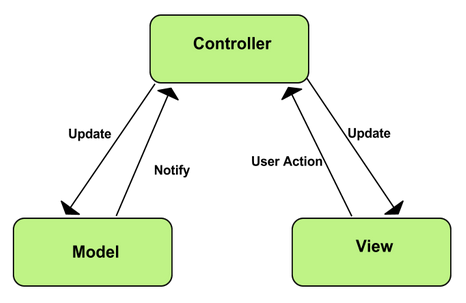
\includegraphics[height=6cm, width=9cm]{img/mvc.png}
\end{center}

\section{Hibernate ORM}

Hibernate ORM\cite{Hibernate} is referred usually too as Hibernate for short. Hibernate is an Object Relational Mapping framework which is what ORM stands for. ORM is a technique for mapping objects, in our case, mapping instances of Java classes and relating them to tables and columns in our chosen database. There instances of Java classes are known as POJO's or plain ordinary Java objects. Mapping of the objects to columns and tables in Hibernate is done through XML\cite{HibernateXML}\cite{XML} files or more recently through annotations\cite{HibernateAnnotations}. Hibernate XML files can be generated through Eclipse but if column names differ from field names you will find yourself spending a lot of time manually editing these files. This leads a lot of margin for error and leads to a lot of overhead. E.g Manually assigning primary keys, fields and making sure relations are properly defined. 
\noindent \newline \newline Below is an example of this 

\begin{center}    
	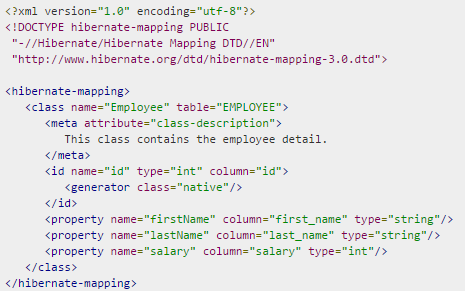
\includegraphics[height=9cm, width=14cm]{img/hibernatemapping.png}
\end{center}

Annotations, which were brought in by newer versions of Hibernate scraps the ideas of these XML files and makes things alot easier. Instead of mapping out every member variable for a class you can set up mapping now with a few simple annotations

\begin{center}    
	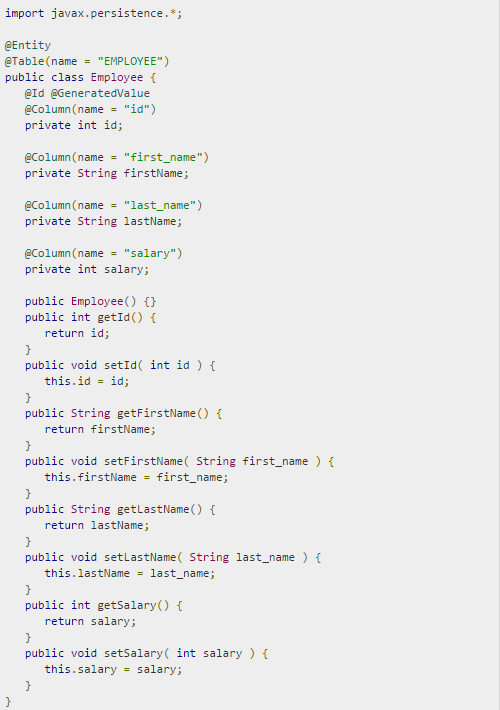
\includegraphics[height=18cm, width=12cm]{img/hibernateclass.png}
\end{center}

Hibernate also has a configuration file which must be set up. This holds connection information for the database and other settings.

\begin{center}    
	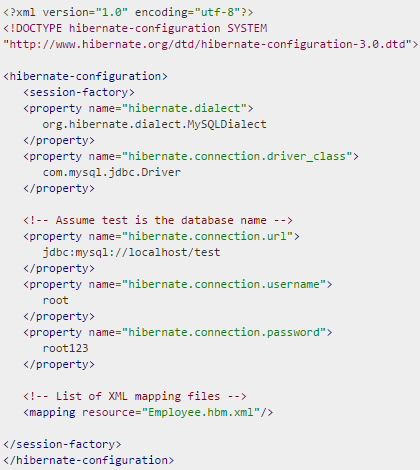
\includegraphics[height=14cm, width=13cm]{img/hibernatesettings.png}
\end{center}

Originally experimenting and learning was done using version 3 of Hibernate and used Hibernates Object Relational Mapping using XML files. These files are in typical XML format. To use this method of mapping must define the mapped files in the hibernate configuration file, if not when you try to commit the object to the database an exception is thrown. Furthermore any errors in the XML or mistypes in the mapping will stop any operations using this object.

We were successful with implementing some basic CRUD methods (Create,Read,Update and Delete). This required alot of manual configuration with the XML files. The Eclipse IDE which we used allows you to generate these hbm.xml files but they were not always correct. You must take into account that when generating these xml mapping files Eclipse has no knowledge of the database. If for whatever reason you have configured your column names in the database differently you will have configure them manually for every POJO with mapping in your project. Due to this it was best to keep field names in the POJO classes the same in both the project and the database. Hibernate will also try to generate keys and guess which field is key in the POJO or not even find the key at all. Usually the autogeneration just looked for a field called "id". Due to this you'll have to manually configure the id and it's relationship. Another major overhead of autogenerating these files is having to generate a mapping file for each class dependant on the current class you are generating the mapping for. The more relations an object has, the more files you have to configure and this was very tedious. The margin for error was high, autogeneration lead to mistakes and overall it was very rigid. This lead to very slow workflow because the IDE wouldn't return the location of errors in these files and would leave you guessing alot of the time. This experience stood to us as we now knew how to commit the objects to the database correctly. Once we had information going into the database and coming back we went back into another research phase.

Upon researching more we found alot of information about using annotations with Hibernate and that in recent version they had removed away from the traditional method of mapping using the hbm.xml files. In the case where future changes might be made to the work we have worked on it was best to research annotations more as it seemed it could speed up development and remove the need for those mapping files. We moved up a version of Hibernate and discovered Hibernate JPA Annotations. While we succeeded in getting this XML mapping working Hibernate Annotations drastically changed the workflow. Annotations removed the need for hbm.xml files and you could simply add simple annotations to the POJO class.

Creating the actual database from these classes had to be done manually. Hibernate does have the capacity to do this automatically based off the current classes but this lead to issues. The particular component was "hibernate.hbm2ddl.auto" this is called in the spring.xml file which serves as configuration file for server connection strings and to name the annotated or mapped classes. The reason this wasn't used was because it would force the generation of tables for classes we didn't use and forced the generation of tables for interfaces strangely. Some of these tables weren't needed so the tables that Hibernate generated for us were used as a guide more than anything. Using Hibernate we also found that Hibernate would look for those interface tables, this really complicated things, we only required a minimal amount of tables in the database. Due to this the decision was taken to ignore some of the composition with the POJO's and manage them manually. So in our case the class DefaultOrientationService held a set of Reviews in a ReviewSet. It was much cleaner to assign a review set id to a review and store the reviews individually that way. This solution removed the need for all these interval tables in the database. The idea was to keep our footprint on the database as light as possible. In the end we reduced the amount of tables needed in the database down too four relatively simple tables.

\section{HTML and CSS, JavaScript/jQuery}

We didn't use much HTML\cite{HTML} and CSS\cite{CSS} because the sidebars and navigation bars around the content would later be updated to the style created by RoamPA's team. A simple Bootstrap\cite{Bootstrap} was used as a template and was later removed. All the functionality of the map was achieved using Google Maps Places API\cite{GoogleMaps}. This was all done through JavaScript\cite{ECMAS}. Anything that needed to be done by the back-end was sent through to the proper MVC routes on the server controller by using JavaScript.

\section{Review Systems Literature}

\subsection{Word of Mouth Model}
In the context of the time span of computing, Word of Mouth (WOM) has long been shown to be efficacious and an important source of information when consumers wish to make purchasing decisions\cite{Nielsen}. The usage of Word of Mouth as a marketing tool dates back to, at least, the 1970s, after psychologist George Silverman created his 'Word of Mouth Model' after observing focus groups of physicians discussing pharmaceutical products~\cite{WOM}. Here he found that within a focus group the positive opinion of one physician could sway other members of the group who had previously been sceptical, and even the opinions of those whose patients had had negative experiences with a particular drug.

With the rapid proliferation of digital services that allow consumers to review services online this model is now applied as an Electronic Word of Mouth (eWOM), in 2008 Nielsen Online found that 81\% of online shoppers read online reviews from other customers and 71\% agreed that these reviews made them more comfortable in purchasing the product, in comparison only 14\% sought out reviews from an established source~\cite{Nielsen}. In the case of tourism B. Brown of the University of Glasgow concluded that tourists will use online reviews as a way to "pre-visit" locations~\cite{Brown}.

Many sites and web platforms supply the user with the ability review services or goods, however, the quality and quantity of these reviews vary greatly~\cite{Zhang}.

\subsection{Existing Research}
We know that in the field of traditional marketing, by 'Word of Mouth', that the perceived expertise of the reviewer correlates to how likely it is that the receiver will pay attention to the information on offer~\cite{Bansal}. Given that most reviews online are anonymous or tied to identities which the receiver of the review knows nothing about this perceived expertise must be attained in other ways:

Lopez et al\cite{Lopez} performed research on the \emph{yelp.com} platform comparing the 'usefulness' rating of reviews to the traditional WOM model, and found that many of the 'cues' provided by the site to indicate a reviewers credibility or expertise strongly correlated to 'high usefulness' ratings for reviews, particularly in the case of 'local expertise' they found: 

\emph{"Compared to a reviewer with only one review in the neighbourhood, the count of votes increases 14.3\% when the reviewer has more than five reviews in the neighbourhood."}

In the case of Electronic Word of Mouth via online review systems we see that there are some differences in the model;

The critical factor in this context is not necessarily the perceived expertise but the perceived credibility of the source, which can be hard to judge since frequently the source of an eWOM document is anonymous. The receiver of WOM information is more likely to find it credible if the source is known to them\cite{Bart}, however this is rarely the circumstance when we are dealing with online reviews and eWOMs, to offset this many eWOM aggregators apply ratings systems for the reviews themselves\cite{Krestel}, however this has it's own challenges and problems, namely that often a simple 'was this review helpful' binary option does not give a good measurement of how credible the source may be. Additionally we can see that new reviews or reviews on niche products are likely to have very few ratings as to their helpfulness\cite{Ghose}. 

Zhang et al proposed a Probabilistic framework for ranking helpfulness of eWOMs, however there were problems when some eWOMs did not have enough user ratings~\cite{Zhang}. There is also some trouble with the self selective nature of the response to this kind of polling as outlined by Sipos et al\cite{Sipos} where they demonstrate that 

\emph{". . . the observed connection between context and voting  behaviour  cannot  be  captured  by  a  cardinal  voting model (Section 3), where users make absolute and independent judgements about helpfulness."}

i.e. the context in which a review is presented influences the polarity of the ratings that it receives.

In their paper, Kim et al\cite{Kim} explored automatically rating reviews by helpfulness without manual user input using a Support Vector Machine regression algorithm relying on the wealth of existing eWOMs from other sites. 

Ammar et al\cite{Ammar} of MIT propose a ranking system based on partial data by combining ordinal (comparison) data and first-order marginal (top preference) data, however this requires two forms of ranking to be carried out by the user, both making comparisons and ranking in order of preference.

Another phenomena that one encounters in the context of Electronic Word of Mouth is 'spam', Lim et al\cite{Lim} define this to be:

\emph{". . . all forms of malicious manipulation of user generated data so as to influence usage patterns of the data"}

This definition would, in some cases, overlap with fraud, and spam need not be malicious in all situations, however, they refer to this as 'review spam' or 'opinion spam' in the context of online reviews, and characterise it as reviewers habitually leaving reviews rating services at a significant deviation from the mean rating for that service. They propose to implement aggregation of the reviewer to detect this behaviour and preserve the integrity of the review system. This approach also seems to suffer from removing the reviews of people who are simply more or less critical than average.

Centeno et al\cite{Centeno} discuss online review system fraud, defining fraud as:

\emph{"The fact of promoting bad entities, or damage the reputation of good entities"} 

They propose a solution to this problem by replacing the standard rating system with a comparison system asking users:

\emph{'Which review do you think users would find more helpful, A or B?'}.

Dubey et al\cite{Dubey} state that due to the vast quantity of reviews on some services that users will only read a small sample of these which may not be representative, they propose a technique of summarising reviews by first clustering them by user rank (which has been outlined above) and then selecting the sections of those reviews which are similar to the others in their cluster. They do not consider this an opinion mining activity as there isn't semantic analysis taking place, merely similarity analysis. This approach has a drawback in that it \emph{". . . sacrifices the immediacy and narrative structure of reviews"}\cite{Lappas} according to Lappas et al of Boston University. 

Jin et al\cite{Jin} recommend a true opinion mining algorithm which clusters reviews by ordinal rank (rank they give to the service) and then using the service characteristics as keywords to perform the opinion mining. The ordinal clustering allows for both detecting customers fulfilled and unfulfilled needs without need to resort to elaborate semantic analysis.

Lappas et al\cite{Lappas} also state that ranking by 'usefulness' or 'importance' as we saw earlier \emph{"Leads to redundant or non-representative summaries"}, they propose a system which selects a subset of reviews in those cases where there are a number that it is infeasible for the user to scan through manually, and use a similar technique to that of Jin et al to select reviews that deal with key features of the service. Their aim is to maintain the statistical properties of the superset in their subset with regards to both ordinal distribution and feature discussion.

Ghose et al\cite{Ghose} also propose an opinion mining approach but they tune their algorithm to maximise economic results, i.e. promoting the reviews which have the largest effect on sales. Here they propose to assign the review a Subjectivity/Objectivity score by using text mining to determine whether the review is factual, based on features of the service, or sentimental, based on a personal description of the service or experience with the service. They then analysed these subjectivity values against economic impact. The findings here were not conclusive, however they did find a correlation between reviews that combined objectivity and subjectivity with higher 'usefulness' scores from users.

\subsection{Analysis}
What becomes clear from the predominance of the literature is that this field of research is booming alongside the prevailing business model of service aggregation with many business being based on the disruptive business plan of 'man in the middle, service aggregator, platform' a la \emph{Uber}, \emph{AirBnB}, \emph{TripAdvisor} etc. All of these platforms feature user reviews prominently and the amount of raw user content being produced mandates aggregation of some sort. 

As we have seen there are many competing approaches to this problem each with downsides, whether they be functional or in difficulty of implementation, or both. It is apparent that the approaches to solve the problem have continued to evolve as the commonality of the problem increases. The simplest approaches are allowing users to rate services and simply displaying those reviews in some order, from there reviews are reviewed by other users, reviewers build up aggregate scores to determine credible reviewers, and then there are the statistical approaches, and finally the sentiment mining and machine learning approaches.

We also see from the Lim et al paper\cite{Lim} and the Centeno et al\cite{Centeno} paper that there are pitfalls that any review system must deal with beyond normal security, the system also has to deal with abnormal user behaviour to ensure integrity and value to other users.

\subsection{Literature Conclusion}
In conclusion, the literature seems to indicate that a review system must be designed with context in mind, some solutions are better suited to environments where there is an abundance of user data, in the form of reviews and rankings of those reviews, which need to be aggregated, while others are better suited to environments with a scarcity of reviews and rankings. In addition we see that some environments can lend to enhanced 'perceived expertise' (which translates to perceived credibility in an electronic context) from the traditional Word of Mouth model, in that an environment can, at least, 'confirm' that the reviewer is an actual customer (i.e. confirmed purchase on a retailer site). Other environments allow anyone to leave reviews in which makes the case for any given reviewers perceived credibility is harder to make. In the latter situation, the possibility of fraud and undesirable user behaviour (i.e. spamming) is of more concern, so the recommendations of \cite{Lim}Lim et al and \cite{Centeno}Centeno et al are more important.

It also appears to be of some significance to provide cues as to a users credibility, that is; their level of expertise in a geographical area, how useful their reviews are to other users and so on\cite{Lopez}.


\chapter{System Design}

The system consists of many elements and dependencies working together on a Tomcat Server. Developing this system required understanding the defacto standard for developing a Spring MVC application. Spring MVC dictated the of the structure of the application and because this is constraint of the environment the design and flow of data must follow Spring's architectural pattern.

\section{MySQL}

Starting from the bottom of the system design, we knew from our specifications that we would be using a MySQL database. Initially we had tested with mockup objects and then later with MySQLite but the release was to use MySQL. 

MySQL is a relational database that has been around for 20 years, it provides atomicity and is used widely in the industry. It made sense to use a relational database with the application because we are dealing with easily related data. An example of this is evident in our database e.g An orientation service has a review set which relates to views about an establishment. Furthermore these reviews has individual likes and dislikes on them. All of this data is closely related to each other and using a MySQL database made sense to use. Working with this database was also good because the connectors and database drivers between MySQL and Hibernate existed due to MySQL's popularity.

\section{Hibernate and SpringMVC}

Hibernate is a framework that can work closely with SpringMVC to facilitate the transfer of information too and from the database. Hibernate deals with object relational mapping. In Hibernate's case, object relational mapping is the mapping of JAVA objects to databases and columns. Hibernate was key to making the application function.   





Spring MVC implements the Model View Controller pattern as mentioned earlier. This meant we couldn't access data directly from the database or HTML pages without dealing with a controller that deals with all of the users requests.

SpringMVC has it's own slightly altered version of this. It works off the same principals just with a more in-dept controller dealing with our users request.

\begin{center}    
	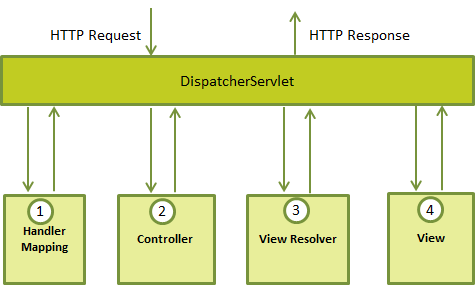
\includegraphics[height=7cm, width=12cm]{img/springmvc.png}
\end{center}

\begin{itemize}	
\item{ After receiving an HTTP request, DispatcherServlet consults the HandlerMapping to call the appropriate Controller.}
\item{ The Controller takes the request and calls the appropriate service methods based which kind of method used, e.g GET or POST method. The service method will set model data based on defined business logic and returns view name to the DispatcherServlet.}
\item{ The DispatcherServlet will take help from ViewResolver to pickup the defined view for the request.}
\item{Once the view is finalized, The DispatcherServlet passes the model data to the view which is finally rendered on the browser.}
\end{itemize}	

It was very important to the project to understand this MVC concept

\chapter{System Evaluation}
As many pages as needed.
\begin{itemize}
\item Prove that your software is robust. How? Testing etc. 
\item Use performance benchmarks (space and time) if algorithmic.
\item Measure the outcomes / outputs of your system / software against the objectives from the Introduction.
\item Highlight any limitations or opportunities in your approach or technologies used.
\end{itemize}

\chapter{Conclusion}
About three pages.

\begin{itemize}
\item Briefly summarise your context and objectives (a few lines).
\item Highlight your findings from the evaluation section / chapter and any opportunities identified.
\end{itemize}



%= - 1 Apache Tomcat ~ http://tomcat.apache.org/ 
%= - 2 Hibernate ORM~ http://hibernate.org/
%= - 3 Spring MVC ~ https://spring.io/
%= - 4 JSP Pages ~ https://docs.oracle.com/javaee/5/tutorial/doc/bnagy.html
%= - 5 ModelViewController Explained ~ http://blog.codinghorror.com/understanding-model-view-controller/ 
%= - 6 SpringMVC ~ http://www.tutorialspoint.com/spring/spring_web_mvc_framework.htm
%= - 7 Hibernate Example ~ http://www.tutorialspoint.com/hibernate/hibernate_mapping_files.htm
%=  http://puu.sh/og17d/1dde409ae4.png
%= - 8 Hibernate Annotations ~ http://www.tutorialspoint.com/hibernate/hibernate_annotations.htm
%= - 9 Hibernate Configuration ~ http://www.tutorialspoint.com/hibernate/hibernate_configuration.htm
%= - 10 OpenStreetMap ~ http://wiki.openstreetmap.org/wiki/API
%= - 11 Leaflet ~ http://leafletjs.com/
%= - 12 Bing Maps ~ https://www.microsoft.com/maps/choose-your-bing-maps-API.aspx
%= - 13 Example Google Places ~ https://developers.google.com/places/javascript/
%= - 14 Hibernate JPA Annotations ~ https://docs.jboss.org/hibernate/stable/annotations/reference/en/html_single/
%= - API definition https://en.wikipedia.org/wiki/Application_programming_interface
%= - IDE definition http://searchsoftwarequality.techtarget.com/definition/integrated-development-environment
%= - Eclipse https://eclipse.org/